%!TEX root = labreport.tex
%%%%%%%%%%%%%%%%%%%%%%%%%%%%%%%%%%%%%%%%%%%%%%%%%%%%%%%%%%%%%%%%%%%%%%%%%%%

\documentclass[sigconf]{acmart}

\usepackage{booktabs} % For formal tables
\usepackage{amsmath}

% Copyright
\setcopyright{none}
%\setcopyright{acmcopyright}
%\setcopyright{acmlicensed}
%\setcopyright{rightsretained}
%\setcopyright{usgov}
%\setcopyright{usgovmixed}
%\setcopyright{cagov}
%\setcopyright{cagovmixed}


% DOI
% \acmDOI{10.475/123_4}

% ISBN
% \acmISBN{123-4567-24-567/08/06}

%Conference
\acmConference[SEEMOO PhySec (Lab RDS) 2017/18]{Physical Layer Security
in Wireless Systems (Lab RDS) 2017/18}{February 2018}{Darmstadt, Germany}

\acmYear{2018}
\copyrightyear{2018}

% \acmArticle{4}
% \acmPrice{15.00}

\settopmatter{printacmref=false}

\begin{document}
\title{Reactive Jamming}

% Comment out the following for you final document
\subtitle{Lab Report}



\author{Daniel May}
\author{Simon Schmitt}
\affiliation{%
  \institution{Technische Universtit\"at Darmstadt}
}
\email{daniel\_nicolas.may@stud.tu-darmstadt.de}
\email{simon\_johannes.schmitt@stud.tu-darmstadt.de}

% The default list of authors is too long for headers.
\renewcommand{\shortauthors}{Daniel May \& Simon Schmitt}


\begin{abstract}
%  Answer the following questions with roughly one sentence each:
%
%  One-page summary:
%  \begin{itemize}
%  \item What is the topic of your main seminar paper?
%  \item What problem does it solve?
%  \item Why is that topic/problem important?
%  \item What methodologies do the authors apply?
%  \item What are the main contributions of the paper?
%  \item What are the key findings/results of the paper?
%  \end{itemize}
%  
%  Final seminar paper:
%  \begin{itemize}
%  \item What is your research question?
%  \item Why are that question and your topic important?
%  \item How did you proceed to answer the question?
%  \item What (do you think) is the answer to your question?
%  \item Give an overall opinion on your topic.
%  \item If you have results, describe them.
%  \item What is the impact of the answers to your questions?
%  \end{itemize}
This lab report presents the creation of an reactive jammer. We will describe how the frame handling
works on the WARP and how it can be used to suppress individual targeted devices or communications
respectively. At the end of this report we evaluate the performance of our jammer and discuss
possible improvements.


\end{abstract}

\maketitle

\section{Introduction}
Wireless signals, as they are used in most of today's analog or digital communications, are very
sensitive and affectable by the environment. Signals with the same frequency can interfere and
suppress each other. This effect is typically used by jammers to prevent a certain receiver from
decoding a signal. While jamming is typically associated with malicious behaviour or within military
conflicts to hinder an opposing party from exchanging information, there also exist other jamming
schemes, so called friendly jamming. Friendly jamming can be used to protect vulnerable systems from
adversarial actions, e.g., pacemakers that can be wirelessly reprogrammed. More recent work also
demonstrated that secrete key-exchanges can be realized at the physical layer utilizing a jammer.

The objective of this lab was to create a reactive WiFi jammer using the Wireless Open-Access
Research Platform (WARP). WARP is a programmable Software-Defined Radio (SDR) which provides a basic
implementation of the 802.11g WiFi standard. The architecture of the WARP allows to transmit frames
while still receiving a signal. Thus WiFi transmissions containing a certain Medium Access Control (MAC)
address can be analyzed and jammed if they are matching a target address.

In comparison with existing jammers this approach is more precise as it only suppresses the signals
of a certain target, while still allowing the communication of other devices. This also results in
much lower power-consumptions, due to the smaller amount of frames that have to be jammed.

%Write a short paragraph (5-15 lines) on each of the following tasks:
%\begin{itemize}
%\item Motivate your topic in general.
%\item Why is your research question important in that field?
%\item Give one practical example.
%\item To what existing work is your topic related, what has been done there?
%\item What are the (planned) main contributions of your paper? e.g., a
%new attacker model, a summary, a comparison, \dots
%\item Give an outline of the paper: describe each of your (planned)
%sections in one sentence.
%\end{itemize}


\section{Background on the WARP}
In this Section we describe how the frame handling works on the Wireless Open-Access
Research Platform (WARP) and why there are multiple receive and transmit buffers.

The WARP is a transceiver, which means it can be used to send and receive frames respectively. This
is realized with two independent paths of circuits that are connected to a single antenna (1). 
The antenna is followed by a switch (2) to either connect to the transmitter or receiver
path. At the receiving path the incoming frames are directly forwarded to the transceiver module
(4), while the signals leaving this module are amplified to a fixed gain (3). The transceiver module
controls the conversion between the complex baseband signal and the Radio Frequency (RF) using a
quadrature modulator. The next layer (5) contains the Digital-to-Analog and Analog-to-Digital
Converter, which are connected to the chips that implement the 802.11 physical layer (6). Incoming
frames are written into a RX Packet Buffer, while outgoing frames are read from the TX Packet
Buffer. Both buffers represent shared memory that is also accessible by the MicroBlaze processor (7),
which handles the MAC layer of the network interface. Whats special about the WARP, is the fact that
the processor allows to start processing while incoming frames are still being received. This
allows us to implement a reactive jammer. It is only necessary to prepare the frames used for the
jamming signal. Those frames are stored in the TX Packet Buffer and can be send as soon as a
condition matches to the incoming frame.

The JTAG port (9) is used to flash the firmware of the processor and to upload the implementation of
the reactive jammer. Any debugging messages that are written to the standard output can be observed
in a terminal that is connected to the UART to USB port (10).

\begin{figure}[tb!]
	\hfill
	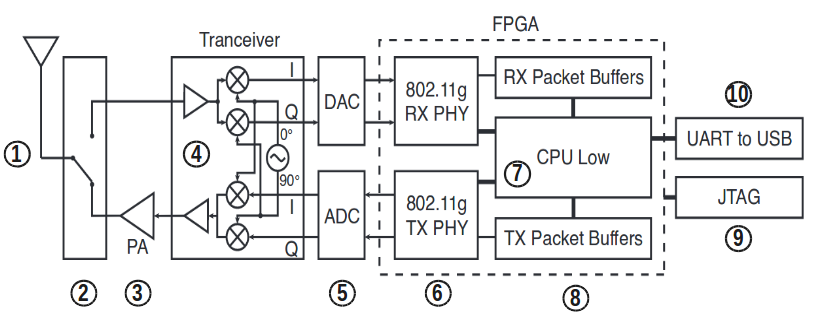
\includegraphics[width=1\linewidth]{block_diagram_warp.png}
	\caption{Block diagram of the 802.11 WARP}
	\label{fig:block_diagram_warp}
\end{figure}

\section{Implementation}

In this Section we describe how a reactive jammer can be implemented using the previous described
Wireless Open-Access Research Platform (WARP). As a development environment we used the Eclipse-based
Xilinx Software Development Kit and Putty as a terminal for the standard output. The logic is
implemented in C and executed by the CPU low of the WARP.

\pagebreak

As a first step we setup the WiFi 802.11 standard and the callback-function that are executed if a
new frame is received or needs to transmitted. 

\begin{verbatim}
	wlan_mac_low_init(WARPNET_TYPE_80211_LOW);

	// ...

	wlan_mac_low_set_frame_rx_callback((void*)frame_receive);
	wlan_mac_low_set_frame_tx_callback((void*)frame_transmit);
\end{verbatim}

In order to check for incoming frames, the\\\texttt{wlan\_mac\_low\_poll\_frame\_rx} function needs to be executed
in a loop. 

\begin{verbatim}
	while(1) {
	    wlan_mac_low_poll_frame_rx();
	}
\end{verbatim}

If the RX PHY received a new frame this function will call the frame\_received function to handle the
reception. Since we are about to implement a reactive jammer, it is of importance that the jamming
signal is sent as soon as the currently received frame can be assigned to a certain transmitter.
Therefore, we add the check for the jamming condition (MAC address of the target system) to the
frame\_received function. If the condition is "true" we create the jamming signal and transmit it
using the frame\_transmit function. Notice that the transmission is started, while still
receiving the targeted signal. As a result the signal gets destroyed for other receivers. To ensure
this happens we have to implement the transmission of our jamming signal right before the call to the
blocking function \texttt{wlan\_mac\_dcf\_hw\_rx\_finish}, since this function blocks the execution of the further
code until the complete frame is received.

If we receive a frame that we want to jam, we need a valid WiFi frame that can be transmitted to jam
the original signal. Since the frames we copied to the TX Packet Buffer of the WARP were apparently
cleared automatically after their transmission, we copy a new one to the Buffer if the above mentioned
condition applies. To create the MAC header we use the predefined mac\_header\_80211 structure
and set the fields to the following values, where the \texttt{mac} variable contains our MAC address.

\begin{verbatim}
	mac_header_80211 header;
	header.frame_control_1 = MAC_FRAME_CTRL1_SUBTYPE_DATA;
	header.frame_control_2 = MAC_FRAME_CTRL2_FLAG_FROM_DS;
	header.duration_id = 0;
	memcpy(header.address_1, mac, 6);
	memcpy(header.address_2, mac, 6);
	memcpy(header.address_3, mac, 6);
	header.sequence_control = 0;
\end{verbatim}

Beyond this, the WARP needs some further information for each frame with details about its transmission
that has to be stored in the Packet Buffer. For one, there is a predefined structure \texttt{tx\_frame\_info} which
we do not use for our jammer but have to consider when calculating the size of the final block to write into the
buffer. Then follows a header containing information that is used to give the chip on the WARP details about
handling the frame at the physical layer. This contains the transmit power and the antenna interface which
should be used.

In order to know to which address we have to store our MAC header we first need to know the order in which
the parts described above are expected to be in the buffer. First the chip looks for the
\texttt{tx\_frame\_info}, then the physical and finally for the MAC header. Thus we need to sum up the size of
the \texttt{tx\_frame\_info} structure and the physical layer header and add them to the address of the current
packet buffer. To this address we can finally write the MAC header we created above.

\begin{verbatim}
memcpy((TX_PKT_BUF_TO_ADDR(pkt_buf) + 
    PHY_TX_PKT_BUF_PHY_HDR_SIZE + 
    sizeof(tx_frame_info)), 
    &header, 
    sizeof(header));
\end{verbatim}

With this header finished, we still need to write the header for the TX PHY core. Since we want our jammer to
be as effective as possible, we set the transmission power to the maximum and choose the only attached
antenna at port A.

\begin{verbatim}
	set_tx_power(pkt_buf, TX_POWER_MAX_DBM);
	set_tx_ant_mode(pkt_buf, TX_ANTMODE_SISO_ANTA);
\end{verbatim}

Being done with the preparation for the transmission of our jamming frame, we can finally tell the CPU to transmit
our frame.

\begin{verbatim}
	frame_transmit(pkt_buf,WLAN_PHY_RATE_BPSK12,
	    sizeof(header), NULL);
\end{verbatim}

The one thing still missing from our implementation is the analysis of the incoming frame with the check if we
need to jam it. This has obviously to be done before the transmission of the jamming frame.
To lose as little time as possible, we want our receiving function to wait just until the first target MAC address
has been received. Since we know that the thirteenth byte is the beginning of the first MAC address and the
addresses are six byte long, we tell our receiver to wait until the reception of the 19-th byte. In the lab we tried
to do this using an empty \texttt{while} loop, which did not work in practice. We assume that the compiler
removed the empty loop in an optimization. When we added an console output of an empty string, it worked as
expected.

\begin{verbatim}
	while(wlan_mac_get_last_byte_index() <= 19) {
	    xil_printf("");
	}
\end{verbatim}

As soon as these first bytes are received we copy the contents of the RX packet buffer to a \texttt{mac\_header\_80211}
structure variable. The information after the first MAC address is still not valid, but this does not pose a problem
since we are only interested in this MAC address. For reading from the receive buffer we can proceed exactly 
like before with the transmit buffer because they are structured identically.

\begin{verbatim}
	memcpy(&header, ((void *)(RX_PKT_BUF_TO_ADDR(rx_pkt_buf))
	    + PHY_RX_PKT_BUF_PHY_HDR_SIZE
	    + sizeof(rx_frame_info)), sizeof(header));
\end{verbatim}

The only missing part is the actual comparison of the included MAC address and the one we want to jam. We can
access the received address using our \texttt{header} structure variable and compare it to the \texttt{jam\_me\_mac}
address, that contains the address we want to jam.

\begin{verbatim}
	if (wlan_addr_eq(header.address_1, jam_me_mac)) {
\end{verbatim}

In this if block follows the code we wrote to transmit our jamming signal described above. 



\section{Evaluation}
The address we wanted to jam in this lab was in our case \\\texttt{DE:AD:BE:EF:22:22}. Figure \ref{fig:jammings_result}
shows the result when our jammer was turned on while none of the other groups were active. The bars show how many
valid packets containing the corresponding MAC address were received in packets per second at the evaluation netbook. 
The bars for the other addresses stayed always close to 16-17 packets independent of the activity of our jammer. Just
for our target the packet rate dropped to 0 packets per second while our jammer was active and regained the same
value as the other receivers when we switched it off. This shows that our reactive jammer indeed works in practice, where
he can jam all frames to a target MAC address while not noticeable affecting one of the other ones.


\begin{figure}[tb!]
	\hfill
	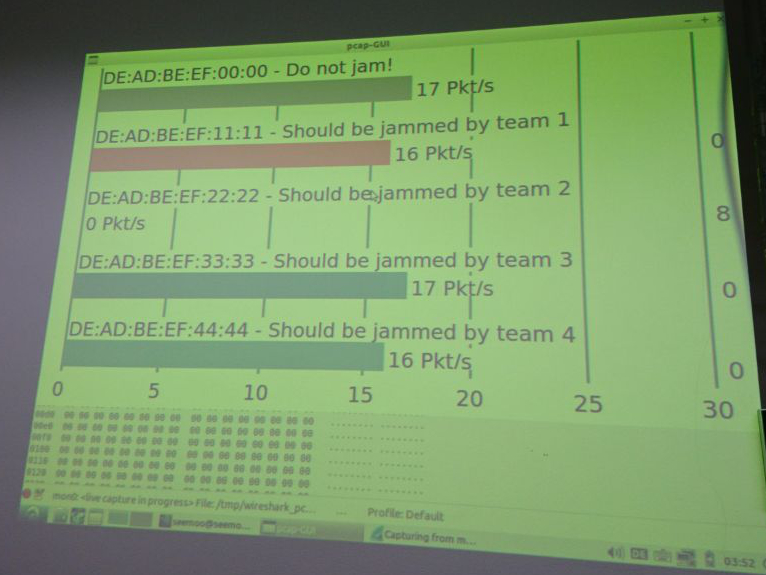
\includegraphics[width=1\linewidth]{jamming_result.jpg}
	\caption{Jamming results using our jammer}
	\label{fig:jammings_result}
\end{figure}



\begin{comment}
\begin{verbatim}
	u32 frame_receive(u8 rx_pkt_buf, u8 rate, u16 length){
		mac_header_80211 header;

		while(wlan_mac_get_last_byte_index() <= 19) {
			xil_printf("");
		}

		memcpy(&header, ((void *)(RX_PKT_BUF_TO_ADDR(rx_pkt_buf)) + 
				PHY_RX_PKT_BUF_PHY_HDR_SIZE + sizeof(rx_frame_info)), 
				sizeof(header));

		if (wlan_addr_eq(header.address_1, jam_me_mac)) {
			is_pushed = 1;
			u8 pkt_buf = 0;
			mac_header_80211 header;
			header.frame_control_1 = MAC_FRAME_CTRL1_SUBTYPE_DATA;
			header.frame_control_2 = MAC_FRAME_CTRL2_FLAG_FROM_DS;
			header.duration_id = 0;
			memcpy(header.address_1, mac, 6);
			memcpy(header.address_2, mac, 6);
			memcpy(header.address_3, mac, 6);
			header.sequence_control = 0;

			memcpy((TX_PKT_BUF_TO_ADDR(pkt_buf) + 
				PHY_TX_PKT_BUF_PHY_HDR_SIZE + 
				sizeof(tx_frame_info)), 
				&header, 
				sizeof(header));
			set_tx_power(pkt_buf, TX_POWER_MAX_DBM);
			set_tx_ant_mode(pkt_buf, TX_ANTMODE_SISO_ANTA);
			frame_transmit(pkt_buf,WLAN_PHY_RATE_BPSK12, sizeof(header),NULL);
		}

		//Blocks until reception is complete
		u32 state = wlan_mac_dcf_hw_rx_finish(); 
		
		// ...
	}
\end{verbatim}
\end{comment}

\section{Conclusion and Take-Away}
In this lab we implemented our own reactive jammer. We started by looking at the Wireless Open-Access Research Platform,
how it works, how we can use it to implement our jammer and which peculiarities we need to consider. Then we implemented
the building of a WiFi frame with a valid MAC header and the additional informations the WARP requires. Finally we added
an analysis of received frames that checks for certain MAC addresses in the headers and included the transmission of our
prepared frame in the case of a match with the address we want to jam. Finally we tried our implementation using a WARP
and could evaluate the success of the reactive jammer.

During the preparation and execution of this .lab we learned how little effort it is to implement and use a jammer in WiFi
networks if given the necessary hardware.



\section{Future Work}
For future work, this implementation of our reactive jammer might be expanded by additional features. For example it would
be possible to offer different options for the frames the jammer should jam. Instead of jamming all frames to one certain
receiver, one might jam only those using certain services or protocols, or combinations of these and the MAC addresses.
To avoid emerging problems with this approach it would also be possible to extend this implementation to an acknowledging
jammer, that fakes acknowledgement messages to the original sender. If a lower power consumption is important, another
option is to look for improvements that improve the jammer in a way so that it does not have to transmit with full power all of
the time without losing too much efficiency. One approach might be to simply try out lower power levels and then measure if
the jamming is still successful, which could be done dynamically while jamming.


\bibliographystyle{ACM-Reference-Format}
%\bibliography{library} 

\end{document}
